\documentclass{beamer}
\mode<presentation>
\usepackage{amsmath}
\usepackage{amssymb}
%\usepackage{advdate}
\usepackage{adjustbox}
\usepackage{subcaption}
\usepackage{enumitem}
\usepackage{multicol}
\usepackage{mathtools}
\usepackage{listings}
\usepackage{url}
\usepackage{minted}
% \usepackage{gvv}

\usepackage{tcolorbox}
\tcbuselibrary{minted,breakable,xparse,skins}



\definecolor{bg}{gray}{0.95}
\DeclareTCBListing{mintedbox}{O{}m!O{}}{%
  breakable=true,
  listing engine=minted,
  listing only,
  minted language=#2,
  minted style=default,
  minted options={%
    linenos,
    gobble=0,
    breaklines=true,
    breakafter=,,
    fontsize=\scriptsize,
    numbersep=8pt,
    #1},
  boxsep=0pt,
  left skip=0pt,
  right skip=0pt,
  left=25pt,
  right=0pt,
  top=3pt,
  bottom=3pt,
  arc=5pt,
  leftrule=0pt,
  rightrule=0pt,
  bottomrule=2pt,
  toprule=2pt,
  colback=bg,
  colframe=orange!70,
  enhanced,
  overlay={%
    \begin{tcbclipinterior}
    \fill[orange!20!white] (frame.south west) rectangle ([xshift=20pt]frame.north west);
    \end{tcbclipinterior}},
  #3,
}


\def\UrlBreaks{\do\/\do-}
\usetheme{Madrid}
\usecolortheme{lily}
\setbeamertemplate{footline}
{
  \leavevmode%
  \hbox{%
  \begin{beamercolorbox}[wd=\paperwidth,ht=2.25ex,dp=1ex,right]{author in head/foot}%
    \insertframenumber{} / \inserttotalframenumber\hspace*{2ex} 
  \end{beamercolorbox}}%
  \vskip0pt%
}
\setbeamertemplate{navigation symbols}{}

\providecommand{\nCr}[2]{\,^{#1}C_{#2}} % nCr 
\providecommand{\nPr}[2]{\,^{#1}P_{#2}} % nPr
\providecommand{\mbf}{\mathbf}
\providecommand{\pr}[1]{\ensuremath{\Pr\left(#1\right)}}
\providecommand{\qfunc}[1]{\ensuremath{Q\left(#1\right)}}
\providecommand{\sbrak}[1]{\ensuremath{{}\left[#1\right]}}
\providecommand{\lsbrak}[1]{\ensuremath{{}\left[#1\right.}}
\providecommand{\rsbrak}[1]{\ensuremath{{}\left.#1\right]}}
\providecommand{\brak}[1]{\ensuremath{\left(#1\right)}}
\providecommand{\lbrak}[1]{\ensuremath{\left(#1\right.}}
\providecommand{\rbrak}[1]{\ensuremath{\left.#1\right)}}
\providecommand{\cbrak}[1]{\ensuremath{\left\{#1\right\}}}
\providecommand{\lcbrak}[1]{\ensuremath{\left\{#1\right.}}
\providecommand{\rcbrak}[1]{\ensuremath{\left.#1\right\}}}
\theoremstyle{remark}
\newtheorem{rem}{Remark}
\newcommand{\sgn}{\mathop{\mathrm{sgn}}}
\providecommand{\abs}[1]{\left\vert#1\right\vert}
\providecommand{\res}[1]{\Res\displaylimits_{#1}} 
\providecommand{\norm}[1]{\lVert#1\rVert}
\providecommand{\mtx}[1]{\mathbf{#1}}
\providecommand{\mean}[1]{E\left[ #1 \right]}
\providecommand{\fourier}{\overset{\mathcal{F}}{ \rightleftharpoons}}
%\providecommand{\hilbert}{\overset{\mathcal{H}}{ \rightleftharpoons}}
\providecommand{\system}{\overset{\mathcal{H}}{ \longleftrightarrow}}
	%\newcommand{\solution}[2]{\textbf{Solution:}{#1}}
%\newcommand{\solution}{\noindent \textbf{Solution: }}
\providecommand{\dec}[2]{\ensuremath{\overset{#1}{\underset{#2}{\gtrless}}}}
\newcommand{\myvec}[1]{\ensuremath{\begin{pmatrix}#1\end{pmatrix}}}
\let\vec\mathbf

\lstset{
%language=C,
frame=single, 
breaklines=true,
columns=fullflexible
}

\numberwithin{equation}{section}

\title{Matgeo Presentation}
\author{Vijaya Sreyas \\ AI24BTech11003 \\ IIT Hyderabad}
\date{\today} 

\begin{document}

\begin{frame}
\titlepage
\end{frame}

\section*{Outline}
\begin{frame}{Contents}
\tableofcontents    
\end{frame}

\section{Problem}
\begin{frame}{Problem Statement}
    Verify if the point $\vec{P}\brak{-2,4}$ lies on a circle of radius $6$ and center $\Vec{C}\brak{3,5}$.
\end{frame}

\section{Solution}
\subsection{Setup and Variable Definitions}
\begin{frame}{Setup and Variable Definitions}
\begin{table}[h!]    
  \centering
  \begin{tabular}[15pt]{ |c|c|c|}
    \hline
    \textbf{Variable} & \textbf{Description} & \textbf{Value}\\ 
    \hline
	$\vec{P}$ & Given Point & $\myvec{-2 \\ 4}$\\
    \hline 
	$\vec{C}$ & Center of circle & $\myvec{3 \\ 5}$\\
    \hline
	$r$ & Radius of circle & $6$\\
    \hline
\end{tabular}
  \caption{Variables and given data}
\end{table}
\end{frame}

\subsection{Circle Equation Setup}
\begin{frame}{Circle Equation Setup}
    We know:
    \begin{align}
        \vec{u} = -\vec{c}, f=\norm{\vec{u}}^2-r^2
        \label{eq:circ-cr}
    \end{align}
    substituting numerical values in \eqref{eq:circ-cr}
    \begin{align}
        u=-\myvec{3 \\ 5}, f=-2
    \end{align}
    The equation of the circle is then obtained as 
    \begin{align}
        \norm{\vec{x}}^2 -2 \myvec{3 \\ 5}^\top \vec{x} -2 &=0
        \label{eq:circ}
    \end{align}
\end{frame}

\subsection{Checking Point Location}
\begin{frame}{Checking Point Location}
    Now, by substituting the point $\vec{P}$ in \eqref{eq:circ}, we can check where $\vec{P}$ is relative to the circle.
    \begin{align}
        &= \norm{\myvec{-2\\4}}^2-2\myvec{3\\5}^\top\myvec{-2\\4}-2\\
        &= 20-28-2\\
        &= -10 < 0
    \end{align}
    $\therefore$ we can say that the point $\vec{P}$ does not lie on the mentioned circle, but rather, inside it.
\end{frame}

\section{Figure}
\begin{frame}{Figure}
\centering
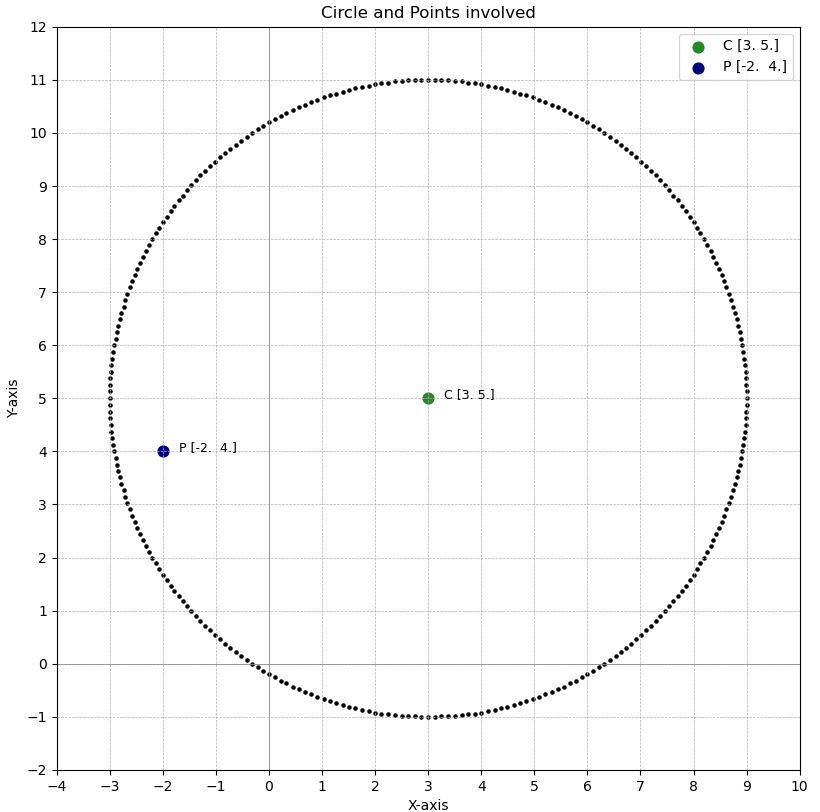
\includegraphics[height=0.9\textheight]{figs/plot.png}
\end{frame}

\section{Codes}
\subsection{Generating points on Circle using C}

\begin{frame}[fragile,allowframebreaks]
\frametitle{Generating points on Circle using C}
\begin{mintedbox}{c}[break at=.8\textheight]
#include <stdio.h>
#include <math.h>

#define NUM_POINTS 300 // Number of points on the circle

void calculateCirclePoints(double x_C, double y_C, double radius, FILE *file) {
    for (int i = 0; i < NUM_POINTS; i++) {
        double angle = 2 * M_PI * i / NUM_POINTS; // Angle in radians
        double x_p = x_C + radius * cos(angle); // xp coordinate
        double y_p = y_C + radius * sin(angle); // yp coordinate
        fprintf(file, "%.2f %.2f\n", x_p, y_p); // Write points to file
    }
}

int main() {
    // Pre-defined P, C coordinates and radius
    double x_C = 3.0; // Center x-coordinate
    double y_C = 5.0; // Center y-coordinate
    double radius = 6.0; // Radius
    double x_P = -2.0; // Point P x-coordinate
    double y_P = 4.0;  // Point P y-coordinate

    FILE *file = fopen("output.txt", "w"); //Open file
    if (file == NULL) {
        perror("Error opening file");
        return 1;
    }
    //Print P, C, and circle points
    fprintf(file, "P %.2f %.2f\n", x_P, y_P);
    fprintf(file, "C %.2f %.2f\n", x_C, y_C);
    calculateCirclePoints(x_C, y_C, radius, file);
    
    fclose(file); // Close the file
    
    return 0;
}

  \end{mintedbox}
\end{frame}
  
\subsection{Plotting the figure using Python}
\begin{frame}[fragile,allowframebreaks]
\frametitle{Plotting the figure using Python}
   \begin{mintedbox}{Python}[break at=.8\textheight]
import sys                                  
sys.path.insert(0, '/home/vijaya-sreyas/IITH/EE1030/matgeo/codes/CoordGeo')
import numpy as np
import numpy.linalg as LA
import matplotlib.pyplot as plt
import matplotlib.image as mpimg

from line.funcs import *
from conics.funcs import *
from triangle.funcs import *
import params
import matplotlib.pyplot as plt

# Read the output from the output.txt file
with open("output.txt", "r") as file:
    output_lines = file.strip().split('\n')

# Get the coordinates for points P and C
point_P = np.array(list(map(float, output_lines[0].split()[1:])))  # P coordinates
point_C = np.array(list(map(float, output_lines[1].split()[1:])))  # C coordinates

# Get the circle points
data = np.array(np.vstack(list(map(lambda line: np.fromstring(line, sep=' '), output_lines[2:]))))

# Separate the circle points into x and y coordinates
xp, yp = data[:, 0], data[:, 1]

# Prepare for plotting
plt.figure(figsize=(8, 8))

# Plot the discrete circle points with smaller size
plt.scatter(xp, yp, color='k', marker='o', s=5)  # Smaller discrete circle points
plt.scatter(point_C[0], point_C[1], color='forestgreen', marker='o', s=60, label=f'C {point_C}')  # Center point (C)
plt.scatter(point_P[0], point_P[1], color='navy', marker='o', s=60, label=f'P {point_P}')  # Point (P)

# Label the points to the right
plt.text(point_C[0] + 0.3, point_C[1], f'C {point_C}', fontsize=9, ha='left')
plt.text(point_P[0] + 0.3, point_P[1], f'P {point_P}', fontsize=9, ha='left')

plt.title('Circle and Points involved')  # Updated title
plt.xlabel('X-axis')
plt.ylabel('Y-axis')

# Set graph limits to ensure all points are visible
plt.xlim(-4, 10)  # X-axis limits
plt.ylim(-2, 12)  # Y-axis limits

# Add gridlines for both odd and even integers
plt.grid(which='both', linestyle='--', linewidth=0.5)
plt.xticks(np.arange(-4, 11, 1))  # Set x ticks for odd and even integers
plt.yticks(np.arange(-2, 13, 1))  # Set y ticks for odd and even integers

plt.gca().set_aspect('equal', adjustable='box')  # Equal aspect ratio
plt.axhline(0, color='grey', lw=0.5)
plt.axvline(0, color='grey', lw=0.5)
plt.legend()

# Save the plot as a PNG file
plt.savefig('plot.png')

#Close the plot
plt.close()
\end{mintedbox}
\end{frame}

\end{document}
